\section{Introduction}
\subsection{Interfaces}
The core of \PolyBoRi is a C++ library. On top of it there exists a Python interface.
Additionally to the Python interface a integration into SAGE was provided by Burcin Erocal.
The main difference is, that \PolyBoRi's built-in Python interface makes use of
the boost library, while the SAGE interface relies on Cython. 
However the wrappers for SAGE and the original Python interface are designed, that it is possible to run the same code under both bindings.

We provide an interactive shell for \PolyBoRi using \ipython for the SAGE
interface~(which is invoked the command~\texttt{sage}) as well as for the
built-in one, which can be accessed by typing~\texttt{ipbori}
at the command line prompt.


In \texttt{ipbori} a global ring is predefined and a set of variables called  $x(0), \ldots, x(9999)$. The default ordering is lexicographical ordering (lp).

In order to follow the instructions of this tutorial a basic knowledge of 
\ipython is necessary. For instance, when  interactively entering programming
blocks (loops, functional definitions), the latter are closed by typing two
additional line breaks.

\subsection{Ring Declarations}
While in ipbori usually a standard ring is predefined,
it is possible to have more advanced ring declarations.
The \lstinline|declare_ring|-function takes two arguments.
The first argument is a list of variables or blocks or variables, and the second is a dictionary where the ring and the variable declarations are written to. The ring always get the name \functionname{r} in that dictionary (the best choice is to use the dictionary of global variables). In addition to that the ring is returned.
\paragraph{Example}
\begin{lstlisting}
In [1]: declare_ring([Block("x",2),Block("y",3)])
Out[1]: <polybori.dynamic.PyPolyBoRi.Ring object at 0x18436f0>

In [2]: r
Out[2]: <polybori.dynamic.PyPolyBoRi.Ring object at 0x18436f0>

In [3]: [r.variable(i) for i in xrange(r.n_variables())]
Out[3]: [x(0), x(1), y(0), y(1), y(2)]

In [4]: declare_ring([AlternatingBlock(["x","y"],2)])
Out[4]: <polybori.dynamic.PyPolyBoRi.Ring object at 0x2370b70>

In [5]: [r.variable(i) for i in xrange(r.n_variables())]
Out[5]: [x(0), y(0), x(1), y(1)]

In [6]: declare_ring([HigherOrderBlock("x", (2, 3))])
Out[6]: <polybori.dynamic.PyPolyBoRi.Ring object at 0x26a86d8>

In [7]: [r.variable(i) for i in xrange(r.n_variables())]
Out[7]: [x(0, 0), x(0, 1), x(0, 2), x(1, 0), x(1, 1), x(1, 2)]

In [8]: declare_ring(["x","y","z"])
Out[8]: <polybori.dynamic.PyPolyBoRi.Ring object at 0x2eb4630>

In [9]: [r.variable(i) for i in xrange(r.n_variables())]
Out[9]: [x, y, z]  
\end{lstlisting}



\subsection{Ordering}
The monomial ordering can be changed by calling
\functionname{change\_ordering}(\functionname{Ordering.code}), where \functionname{code} can be either \functionname{lp} (lexicographical ordering), \functionname{dlex} (degree lexicographical ordering), \functionname{dp\_asc} (degree reverse lexicographical ordering with ascending variable ordering), \functionname{block\_dlex} or \functionname{block\_dp\_asc} (for ordering composed out of blocks in the corresponding ordering). When using block ordering, after changing to that ordering, blocks have to be defined using the \functionname{append\_ring\_block} function.

In contrast to the lexicographical, degree lexicographical ordering, and the degree reverse lexicographical ordering in \Singular, our degree reverse lexicographical ordering has a reverse variable order (the first ring variable is smaller than the second, the second smaller than the third). This is a result of the fact, that efficient implementation of monomial orderings using ZDD structures is quite difficult (and the performance depends on the ordering).
\paragraph{Example}
\begin{lstlisting}
In [1]: r=declare_ring([Block("x",10),Block("y",10)])

In [2]: x(0)>x(1)
Out[2]: True

In [3]: x(0)>x(1)*x(2)
Out[3]: True

In [4]: r = r.clone(ordering=dlex)

In [5]: r(x(0)) > r(x(1))
Out[5]: True

In [6]: r(x(0)) > r(x(1)*x(2))
Out[6]: False

In [7]: r = r.clone(ordering=dp_asc)

In [8]: r(x(0)) > r(x(1))
Out[8]: False

In [9]: r(x(0)) > r(x(1)*x(2))
Out[9]: False

In [10]: r = r.clone(ordering=block_dlex, blocks=[10])

In [11]: r(x(0)) > r(x(1))
Out[11]: True

In [12]: r(x(0)) > r(x(1)*x(2))
Out[12]: False

In [13]: r(x(0)) > r(y(0)*y(1)*y(2))
Out[13]: True

In [14]: r = r.clone(ordering=block_dp_asc)

In [15]: r(x(0)) > r(x(1))
Out[15]: False

In [16]: r(x(0)) > r(y(0))
Out[16]: False

In [17]: r(x(0)) > r(x(1)*x(2))
Out[17]: False

In [18]: r = r.clone(ordering=block_dp_asc, blocks=[10])

In [20]: r(x(0)) > r(y(0))
Out[20]: True

In [21]: r(x(0)) > r(y(0)*y(1))
Out[21]: True
\end{lstlisting}
In this example, we have an ordering composed of two blocks, the first with ten variables, the second contains the rest of variables $y(0), \ldots y(9)$ (per default indices start at 0).

Even, if there is a natural block structure, like in this example, we have to explicit call \lstinline|append_ring_block| in a block ordering to set the start indices of these blocks.

This can be simplified using the variable \lstinline|block_start_hints| created by our ring declaration.

\begin{lstlisting} 
In [1]: declare_ring([
   ...:    Block("x",2),
   ...:    Block("y",3),
   ...:    Block("z",2)],
   ...:    globals())
Out[1]: <polybori.dynamic.PyPolyBoRi.Ring object at 0x1848b10>

In [2]: r.clone(ordering=block_dp_asc, blocks=block_start_hints)

In [3]: block_start_hints
Out[3]: [2, 5]
\end{lstlisting}


Another important feature in \PolyBoRi is the ability to iterate over a polynomial in the current monomial ordering.

\begin{lstlisting}
In [1]: r=declare_ring([Block("x",10),Block("y",10)])

In [2]: f=x(0)+x(1)*x(2)+x(2)

In [3]: for t in f.terms():
   print t
   
x(0)
x(1)*x(2)
x(2)

In [4]: r=r.clone(ordering=dp_asc)

In [5]: for t in r(f).terms():
    print t

x(1)*x(2)
x(2)
x(0)
\end{lstlisting}
%
This is a nontrivial functionality, as the natural order of paths in ZDDs is lexicographical.


\subsection{Arithmetic}
Basic arithmetic is provided in the domain of Boolean polynomials. Boolean Polynomial polynomials are polynomials over $\Ztwo$ where the maximal degree per variable is one.
If exponents bigger than one per variable appear reduction by the field ideal (polynomials of the form $x^2+x$) is done automatically.
\begin{lstlisting}
In [1]: Polynomial(1, r)+Polynomial(1, r)
Out[1]: 0

In [2]: x(1)*x(1)
Out[2]: x(1)

In [3]: (x(1)+x(2))*(x(1)+x(3))
Out[3]: x(1)*x(2) + x(1)*x(3) + x(1) + x(2)*x(3)
\end{lstlisting}

\subsection{Set operations}
In addition to polynomials  \PolyBoRi implements a data type for sets of monomials, called \functionname{BooleSet}.
This data type is also implemented on the top of ZDDs and allows to see
polynomials
from a different angle. Also, it makes high-level set operations possible, which are in most cases faster than operations handling individual terms, because the complexity of the algorithms depends only on the structure of the diagrams.

Polynomials can easily be converted to \functionname{BooleSet}s by using the
member function \lstinline|set()|.
\begin{lstlisting}
In [1]: f=x(2)*x(3)+x(1)*x(3)+x(2)+x(4)

In [2]: f
Out[2]: x(1)*x(3) + x(2)*x(3) + x(2) + x(4)

In [3]: f.set()
Out[3]: {{x(1),x(3)}, {x(2),x(3)}, {x(2)}, {x(4)}}
\end{lstlisting}
%
One of the most common operations is to split the set into cofactors of a
variable. This illustrates the following example.
%
\begin{lstlisting}
In [4]: s0=f.set().subset0(x(2).index())

In [5]: s0
Out[5]: {{x(1),x(3)}, {x(4)}}

In [6]: s1=f.set().subset1(x(2).index())

In [7]: s1
Out[7]: {{x(3)}, {}}

In [8]: f==Polynomial(s1)*x(2)+Polynomial(s0)
Out[8]: True
\end{lstlisting}
%

Even more low-level than operation with \functionname{subset}-methods is the use
of navigators. Navigators  provide an interface to diagram nodes, accessing
their index as well as the corresponding then- and else-branches.

\begin{lstlisting}
In [1]: f=x(1)*x(2)+x(2)*x(3)*x(4)+x(2)*x(4)+x(3)+x(4)+1

In [2]: s=f.set()

In [3]: s
Out[3]: {{x(1),x(2)}, {x(2),x(3),x(4)},
    {x(2),x(4)}, {x(3)}, {x(4)}, {}}

In [4]: x(1).index()
Out[4]: 1

In [5]: s.subset1(1)
Out[5]: {{x(2)}}

In [6]: s.subset0(1)
Out[6]: {{x(2),x(3),x(4)}, {x(2),x(4)}, {x(3)}, {x(4)}, {}}

In [7]: nav=s.navigation()

In [8]: BooleSet(nav,s.ring())
Out[8]: {{x(1),x(2)}, {x(2),x(3),x(4)},
    {x(2),x(4)}, {x(3)}, {x(4)}, {}}

In [9]: nav.value()
Out[9]: 1

In [10]: nav_else=nav.else_branch()

In [11]: nav_else
Out[11]: <polybori.dynamic.PyPolyBoRi.CCuddNavigator
    object at 0xb6e1e7d4>

In [12]: BooleSet(nav_else,s.ring())
Out[12]: {{x(2),x(3),x(4)}, {x(2),x(4)}, {x(3)}, {x(4)}, {}}

In [13]: nav_else.value()
Out[13]: 2
\end{lstlisting}

You should be very careful and always keep a reference to the original object, when dealing with navigators, as navigators contain only a raw pointer as data.
For the same reason, it is necessary to supply the ring as argument, when constructing a set out of a navigator.

The opposite of navigation down a ZDD using navigators is to construct new ZDDs in the same way, namely giving their else- and then-branch as well as the index value of the new node.

\begin{lstlisting}
    
In [1]: f0=x(2)*x(3)+x(3)

In [2]: f1=x(4)

In [3]: if_then_else(x(1),f0,f1)
Out[3]: {{x(1),x(2),x(3)}, {x(1),x(3)}, {x(4)}}

In [4]: if_then_else(x(1).index(),f0,f1)
Out[4]: {{x(1),x(2),x(3)}, {x(1),x(3)}, {x(4)}}

In [5]: if_then_else(x(5),f0,f1)
------------------------------------------------
<type 'exceptions.ValueError'>  Traceback (...) 

/home/user/PolyBoRi/<ipython console> in <module>()

<type 'exceptions.ValueError'>: Node index must be smaller
   than top indices of then- and else-branch.
\end{lstlisting}

It is strictly necessary that the index of the created node is smaller than the index of the branches.
%
%
But also operations on higher levels are possible, like the calculation of the minimal terms (with respect to division) in a~\functionname{BooleSet}:
\begin{lstlisting}
In [1]: f=x(2)*x(3)+x(1)*x(3)+x(2)+x(4)

In [2]: f.set()
Out[2]: {{x(1),x(3)}, {x(2),x(3)}, {x(2)}, {x(4)}}

In [3]: f.set().minimal_elements()
Out[3]: {{x(1),x(3)}, {x(2)}, {x(4)}}
\end{lstlisting}

\subsection{\Groebner bases}
\Groebner bases functionality is available using the function \functionname{groebner\_basis} from polybori.gbcore.
It has quite a lot of options and a exchangeable heuristic.
In principle, there exist  standard settings, but~-- in case an option is not
provided explicitly by the user~-- the active heuristic function
may decide dynamically by taking the ideal, the ordering and the other options into account, which is the best configuration.
\begin{lstlisting}
In [1]: groebner_basis([x(1)+x(2),(x(2)+x(1)+1)*x(3)])
Out[1]: [x(1) + x(2), x(3)]
\end{lstlisting}

There exists a set of default options for \functionname{groebner\_basis}.
They can be seen, but not manipulated via accessing \lstinline|groebner_basis.options|.
A second layer of heuristics is incorporated into the \functionname{groebner\_basis}-function, to choose dynamically the best options depending on the ordering and the given ideal.
Every option given explicitly by the user takes effect, but for the other options the default may be overwritten by the script.
This behaviour can be turned off by calling
\begin{lstlisting}
groebner_basis(I,heuristic=False).
\end{lstlisting}

Important options are the following:
\begin{itemize}
    \item \lstinline|other_ordering_first|, possible values are \pythonconstant{False} or an ordering code.
    In practice, many Boolean examples have very few solutions and a very easy \Groebner basis. So, a complex walk algorithm (which cannot be implemented using the \PolyBoRi data structures) seems unnecessary, as such \Groebner bases can be converted quite fast by the 
    normal Buchberger algorithm from one ordering into another ordering.
    \item \lstinline|faugere|, turn off or on the linear algebra
    \item \lstinline|linear_algebra_in_last_block|, this affects the last block of block orderings and degree orderings. If it is set to \pythonconstant{True} linear algebra takes affect in this block.
    \item \lstinline|selection_size|, maximum number of polynomials for parallel reductions
    \item \lstinline|prot|, turn off or on the protocol
    \item \lstinline|red_tail|, tail reductions in intermediate polynomials, this options affects mainly heuristics. The reducedness of the output polynomials can only be guaranteed by the option \lstinline|redsb|
    \item \lstinline|minsb|, return a minimal \Groebner basis
    \item \lstinline|redsb|, return a reduced \Groebner basis (minimal and all elements are tail reduced)
    \item \lstinline|clean_and_restart_algorithm|, from time to time restart the algorithm to clean the system of non minimal elements
\end{itemize}

\subsubsection{Parallelization}
With a view towards parallel computing \PolyBoRi also has a preliminary support
for concurrent processing of  different strategies. Note, this needs the
pyprocessing module to be installed.
For this purpose the function\\
\functionname{groebner_basis_first_finished} had been established.
Very much like the command \functionname{groebner_basis}
the first argument is assumed to be the system of equations,
which is given as a list of Boolean polynomials.
Further arguments are the options for the different strategies (in form of dictionaries with keyword arguments for \functionname{groebner_basis}).

It returns the result of the variant, which  terminates first.

\begin{lstlisting}
In [1]: from polybori.parallel import groebner_basis_first_finished

In [2]: groebner_basis_first_finished([x(2)*x(1), x(1)+1],
   {'heuristic':False}, {'heuristic': True}) 
Out[2]: [x(2), x(1) + 1]
\end{lstlisting} 
The two option sets~-- with and without heuristic~--
present a reasonable choice, in the case that two CPUs are available, but there
is not much known about the ideal.
Usually the computation time for these settings differ very much:
the heuristic is designed to select the apparently best settings in a very
progressive way.
Indeed, it is not always possible to decide
without further experiments, which option setting would lead to  smallest
computation time. Hence, any a~priori choice will lead to a suboptimal
performance~(like all attempts in this area). 
Because there is much experience behind those heuristic strategies, it will
still help to achieve good results  in many cases. Also, it yields the
best out of the box experience~(as far as it is possible here).
Disabling the heuristics will usually result in an
algorithm, which is much closer to the original Buchberger
algorithm, but without the overhead of the heuristic
functionality itself.

Another important set of alternative option sets consists of computing with and
without (dense) linear algebra.

\begin{lstlisting}
In [1]: from polybori.parallel import groebner_basis_first_finished

In [2]: groebner_basis_first_finished([x(2)*x(1), x(1)+1],
   ...:   {'faugere':False,
   ...:   'linear_algebra_in_last_block': False}, 
   ...:   {'faugere':True,
   ...:   'linear_algebra_in_last_block': True})
Out[2]: [x(2), x(1) + 1]

\end{lstlisting}

This parallelization, i.\,e.\ running different strategies in parallel, seems to be
promising, because it potentially provides a 
nonlinear speedup (higher factor than number of CPUs). This
can also be observed in other domains: for instance, current SAT-solvers 
make use of this by choosing different random seeds.

On the other hand, this approach does not contain any cooperation between the
threads/processes. At best it is just as fast as the best variant. When studying
a particular kind of systems, there is usually a good guess in advance for the
best strategy. In this setting, it would be better to use all available CPUs in
order to apply the guessed variant to suitable subproblems.
The used data structure in \PolyBoRi and the functional approach for handling
them, 
seems to be suited to a cooperative shared memory parallelization. However,
the underlying library \CUDD does not provide any support for that. In this way,
this kind of parallelization, remains to be a challenge for the future.
While the ZDD operations cannot be parallelized easily, the linear algebra
backend using M4RI could make use of several CPUs (when compiled with
appropriate settings). 

\subsubsection{Elimination of variables}

Given Boolean generators $G$ of an ideal $I\subset \Ztwo[x_1,\ldots,x_n,y_1,\ldots,y_m]/\langle x_1^2+x_1,\ldots,x_n^2+x_n,y_1,\ldots,y_m \rangle$
we would like to compute a generating system $H$ of Boolean polynomials, where $$\langle H\rangle=\set{p\in I\vert p \mbox{ can be represented by a (Boolean) polynomial in } \Ztwo[y_1,\ldots,y_m]}.$$
 % (fold)

This can be done as in the classical case despite the field equations using an elimination ordering for $x_1, \ldots, x_n$

\begin{definition}[Elimination orderings]
  Let $R=\Ztwo[x_1,\ldots, x_n, y_1, \ldots y_m]$. An ordering~``$>$'' is called an \emph{elimination ordering} of $x_1, \ldots, x_n$, if $x_i>t$ 
  for every monomial~$t$ in~$K[y_1, \ldots, y_m]$ and every $i=1,\ldots,n$. 
\end{definition}
\paragraph{Example} % (fold)
\label{par:example-elimination}
\begin{lstlisting}
In [1]: declare_ring([Block("x",3),Block("y",3)])
Out[1]: <polybori.dynamic.PyPolyBoRi.Ring object at 0x1848b10>

In [4]: G=[x(0)*x(2)*y(0)*y(1) + y(1)*y(2) + y(1),
   ...:  x(1)*x(2)*y(0)*y(2) + x(0)*x(1)*y(2) + y(1),
   ...:  x(0)*x(1)*x(2)*y(1) + x(1) + y(1)*y(2)]

In [2]: r = r.clone(ordering=block_dp_asc, blocks=block_start_hints)

In [4]: G=[r(poly) for poly in G]

In [5]: H=groebner_basis(G)

In [6]: H
Out[6]: 
[x(0)*y(0)*y(1) + x(0)*y(1) + y(0)*y(1) + y(1),
 x(1) + y(1),
 x(2)*y(1) + x(0)*y(1) + y(1),
 y(1)*y(2) + y(1)]

In [7]: [p for p in H 
    if p.set().navigation().value()>=y(0).index()]
Out[7]: [y(1)*y(2) + y(1)]
\end{lstlisting}

For special cases elimination (depending on the formulation of the equations) elimination of (auxiliary) variables can be done much faster as can be seen in \ref{linear-lexicographical-lead-rewriting-systems}.
% paragraph example (end)


% subsection  (end)$

\section{How to program ef{}f{}iciently}
\label{sec:program-efficiently}
The goal of this section is to explain how to get most performance out of \PolyBoRi using the underlying ZDD structure.
This awareness can be seen on several levels
\begin{itemize}
    \item ZDD unaware, pure algebraic programming 
    \item low level friendly programming
    \item replacing algebraic operations by (a composition of) set operations
    \item decision-diagram style recursive programming without caching
    \item decision-diagram style recursive programming with caching
    \item using ZDDs for many other things than polynomial arithmetics
\end{itemize}
\subsection{Low level friendly programming}
\label{low-level-friendly}
\PolyBoRi is implemented as layer over a decision diagram library (\CUDD at the moment).

In \CUDD every diagram node is unique: If two diagrams have the same structure, they are in fact identical (same position in memory).
Another observation is, that \CUDD tries to build a functional style API in the C programming language. This means, that no data is manipulated, only new nodes are created.
Functional programming is a priori very suited for caching and multithreading (at the moment however threading is not possible in \PolyBoRi).
The $\ite$-operator is the most central function in CUDD. It takes two nodes/diagrams $t$, $e$ and an index $i$ and creates a diagram with root variable $i$ and
then-branch $t$, else-branch $e$. It is necessary that the branches have root variables with bigger index (or are constant).
It creates either exactly one node, or retrieves the correct node from the cache.
Function calls which come essentially down to a single $\ite$ call are very cheap.

For example taking the product $
    {x_{1}} \boolemult (x_2\boolemult(x_3\boolemult (x_4\boolemult x_5)))
$
 is much cheaper than $
    ((((x_1 \boolemult x_2)\boolemult x_3)\boolemult x_4)\boolemult x_5)$.

In the first case, in each step a single node is prepended to the diagram, while in the second case, a completely new diagram is created.
The same argument would apply for the addition of these variables.
This example shows, that having a little bit background about the data structure, it is often possible to write code, that looks as well algebraic as provides good performance.

\subsection{Replace algebra by set operations}
Often there is an alternative description in terms of set operations for algebraic operations, which is much faster.

\subsubsection{Construct power sets}
An example for this behaviour is the calculation of power sets (sets of monomials/polynomials containing each term in the specified variables).
The following code constructs such a power set very inefficiently for the first three variables:
\begin{lstlisting}
sum([x(1)**i1*x(2)**i2*x(3)**i3 
    for i1 in (0,1) 
    for i2 in (0,1) 
    for i3 in (0,1)])
\end{lstlisting}
The algorithm has of course exponential complexity in the number of variables.
The resulting ZDD however has only as many nodes as variables.
In fact it can be constructed directly using the following function (from specialsets.py).
\begin{lstlisting}
def power_set(variables):
    if not variables:
        return BooleConstant(1)
    variables=sorted(set(variables),reverse=True,key=top_index)
    res=Polynomial(1, variables[0].ring()).set()
    for v in variables:
        res=if_then_else(v,res,res)
    return res
\end{lstlisting}
Note, that we switched from polynomials to Boolean sets. We inverse the order of variable indices for iteration to make the computation compatible with the principles in \ref{low-level-friendly} (simple $\ite$ operators instead of complex operations in each step).

\subsubsection{All monomials of degree d}
\label{all-monomials-set-operations}
The following function constructs the complete homogeneous polynomial/BooleSet containing all possible monomials of degree $d$.
\begin{lstlisting}
def all_monomials_of_degree_d(d,variables):
    if d==0:
        return BooleConstant(1)
    
    if not variables:
        return []
    variables=sorted(set(variables),reverse=True,key=top_index)

    m=variables[-1]
    for v in variables[:-1]:
        m=v+m
    m=m.set()
    i=0
    res=Polynomial(variables[0].ring().one()).set()
    while(i<d):
        i=i+1
        res=res.cartesian_product(m).diff(res)
    return res
\end{lstlisting}
We use the set of all monomials of one degree lower using the cartesian product with the set of variables and remove every term, where the degree did not increase (boolean multiplication: $x^2=x$).
\subsection{Direct constructions of diagrams}
Sometimes, it is possible to construct the decision diagram directly, as it is theoretically known, how it looks like.
In the following, we construct the same polynomial as in \ref{all-monomials-set-operations} directly by elementary \lstinline|if_then_else| operations. This will save much recursion overhead.
\begin{lstlisting}
def all_monomials_of_degree_d(d, variables):
    variables=Monomial(variables)
    variables=list(variables.variables())
    if not variables:
        assert d==0
        return BooleConstant(1)
    ring = variables[0].ring()
    if d>len(variables):
        return Polynomial(0, ring)
    if d<0:
        return Polynomial(1, ring)

    deg_variables=variables[-d:]
    #this ensures sorting by indices
    res=Monomial(deg_variables)

    for i in xrange(1, len(variables)-d+1):
        deg_variables=variables[-d-i:-i]
        res=Polynomial(res)
        nav=res.navigation()
        navs=[]
        while not nav.constant():
            navs.append(BooleSet(nav,ring))
            nav=nav.then_branch()
        acc=Polynomial(1, ring)
        for (nav, v) in reversed(zip(navs, deg_variables)):
            acc=if_then_else(v, acc, nav)
        res=acc
    return res.set()
\end{lstlisting}

\subsection{Case study: Graded part of a polynomial}
In the following we will show five variants to implement a function, that computes the sum of all terms of degree $d$ in a polynomial $f$.

\subsubsection{Simple, algebraic solution}
\begin{lstlisting}
def simple_graded(f, d):
    return sum((t for t in f.terms() if t.deg()==d))   
\end{lstlisting}
This solution is obvious, but quite slow.

\subsubsection{Low level friendly, algebraic solution}
\begin{lstlisting}
def friendly_graded(f, d):
    vec=BoolePolynomialVector()
    for t in f.terms:
        if t.deg()!=d:
            continue
        else:
            vec.append(t)
    return add_up_polynomials(vec)
\end{lstlisting}
We leave it to the heuristic of the \functionname{add\_up\_polynomials} function how to add up the monomials. For example a divide and conquer strategy is quite good here.

\subsubsection{Highlevel with set operations}
\begin{lstlisting}
def highlevel_graded(f,d):
    return Polynomial(
        f.set().intersect(
            all_monomials_of_degree_d(
                d,f.vars_as_monomial())))
\end{lstlisting}
This solution build on the fast intersection algorithm and decomposes the task in just two set operations, which is very good.

However it can be quite inefficient, when f has many variables.
This can increase the number of steps in the intersection algorithm (which takes with high probability the else branch of the second argument in each step).

\subsubsection{Recursive}
The repeated unnecessary iteration over all variables in $f$ (during the \functionname{intersection} call in the last section) can be avoided by taking just integers as second argument for the recursive algorithm (in the last section this was \functionname{intersection}).

\begin{lstlisting}
def recursive_graded(f,d):
    def do_recursive_graded(f,d):
        if f.empty():
            return f
        if d==0:
            if Monomial(f.ring()) in f:
                return Polynomial(1, f.ring()).set()
            else:
                return BooleSet(f.ring())
        else:
            nav=f.navigation()
            if nav.constant():
                return BooleSet()
            return if_then_else(
                nav.value(),
                do_recursive_graded(
                    BooleSet(
                        nav.then_branch(),
                        f.ring()),d-1),
                do_recursive_graded(
                    BooleSet(
                        nav.else_branch(),
                        f.ring()),d))
    return Polynomial(
        do_recursive_graded(f.set(),d))
\end{lstlisting}
Recursive implementations are very compatible with our data structures, so are quite fast. However this implementation does not use any caching techniques. \CUDD recursive caching requires functions to have one, two or three parameters, which are of ZDD structure (so no integers).
Of course we can encode the degree $d$ by the $d$-th Variable in the Polynomial
ring.

\subsubsection{Decision-diagram style recursive implementation in \PolyBoRi}
The C++ implementation of the functionality in \PolyBoRi is given in this section, which is recursive and uses caching techniques.
{
\lstset{language=C++}
\begin{lstlisting}
// determine the part of a polynomials of a given degree
template <class CacheType, class NaviType, 
class DegType, class SetType>
SetType
dd_graded_part(const CacheType& cache, NaviType navi, DegType deg,  
               SetType init) {


  if (deg == 0) {
    while(!navi.isConstant())
      navi.incrementElse();
    return SetType(navi);
  }

  if(navi.isConstant())
    return SetType();

  // Look whether result was cached before
  NaviType cached = cache.find(navi, deg);

  if (cached.isValid())
    return SetType(cached);

  SetType result = 
    SetType(*navi,  
            dd_graded_part(cache, 
                navi.then_branch(), deg - 1, init),
            dd_graded_part(cache, 
                navi.else_branch(), deg, init)
            );

  // store result for later reuse
  cache.insert(navi, deg, result.navigation());

  return result;
}
\end{lstlisting}}
\lstset{language=[IPython]Python}
The encoding of integers for the degree as variable is done implicitly by our cache lookup functions.

\subsection{Case study: Evaluation of a polynomial}

\subsubsection{Substitute a single variable $x$ in a polynomial by a constant $c$}

Given a Boolean polynomial $f$, a variable $x$ and a constant $c$, we want to plug in the constant $c$ for the variable $x$.

\paragraph{Naive approach}
The following code shows how to tackle the problem, by manipulating individual terms.
While this is a very direct approach, it is quite slow.
The method \functionname{reducible_by} gives a test for divisibility.
\begin{lstlisting}
def subst(f,x,c):
    if c==1:
        return sum([t/x for t in f.terms() 
            if t.reducible_by(x)])+\
            sum([t for t in f.terms() 
                if not t.reducible_by(x)])
    else:
        #c==0
        return sum([t for t in f.terms() 
            if not t.reducible_by(x)])

\end{lstlisting}

\paragraph{Solution 1: Set operations}
In fact, the problem can be tackled quite efficiently using set operations.
\begin{lstlisting}
def subst(f,x,c):
   i=x.index()
   c=BooleConstant(c) # if c was int is now converted mod 2, 
   #so comparison to int(0) makes sense
   s=f.set()
   if c==0:
       #terms with x evaluate to zero
       return Polynomial(s.subset0(i))
   else:
       #c==1
       return Polynomial(s.subset1(i))+Polynomial(s.subset0(i))    
\end{lstlisting}

\paragraph{Solution 2: Linear Lexicographical Lead rewriting systems}
On the other hand, this linear rewriting forms a rewriting problem and can be solved by calculating a normal form against a \Groebner 
basis.
In this case the system is $\{x+c\} \cup \{\explfieldequations\}$ (we assume that $x=x_i$ for some $i$).
For this special case, that all Boolean polynomials have pairwise different linear leading terms w.\,r.\,t. lexicographical ordering,
there exist special functions.

First, we encode the system $\{x+c\}$ into one diagram
\begin{lstlisting}
d=ll_encode([x+c])    
\end{lstlisting}
%
This is a special format representing a set of such polynomials in one diagram, which is used by several procedures in
\PolyBoRi.
Then we may
reduce~$f$ by this rewriting system
\begin{lstlisting}
ll_red_nf_noredsb(f,d)  
\end{lstlisting}
%
%
This can be simplified in our special case in two ways.
\begin{enumerate}
    \item If our system consists of exactly \textbf{one} Boolean polynomial,
    \lstinline|ll_encode| does essentially  a type conversion only (and much overhead).
    This type conversion can be done implicitly (at least using the
\lstinline|boost::python|-based  interface \lstinline|ipbori|).

    So you may call
\begin{lstlisting}
ll_red_nf_noredsb(f,x+c)  
\end{lstlisting}
%
    In this case, there is no need for calling \lstinline|ll_encode|.
    The second argument is converted implicitly to BooleSet.
    \item A second optimization is to call just
\begin{lstlisting}
ll_red_nf_redsb(f,x+c)
\end{lstlisting}
    %
    Note, that $\{x+c\}$ is a reduced Boolean \Groebner basis: Equivalently \[
        \{x+c,\explfieldequations\}\backslash \{x^2+x\}
    \] is a reduced 
\Groebner 
basis).
\end{enumerate}



\subsubsection{Evaluate a polynomial by plugging in a constant for each variable}
    We want to a polynomial
    $f(x_1,\ldots, x_n)$
    by
    $x_i\mapsto c_i$, where
    $c_1,\ldots, c_n$ are constants.

\paragraph{Naive approach}
First, we show it in a naive way, similar to the first solution above.

\begin{lstlisting}
def evaluate(f,m):
    res=0
    for term in f.terms():
        product=1
        for variable in term.variables():
            product=m[variable]*product
        res=res+product
    return Polynomial(res)
\end{lstlisting}


\paragraph{Solution 1: $n$ set operations}
The following approach is faster, as it does not involve individual terms, but set operations

\begin{lstlisting}
def evaluate(f,m):
   while not f.constant():
       nav=f.navigation()
       i=nav.value()
       v=Variable(i)
       c=m[v]
       if c==0:
           #terms with x evaluate to zero
           f=Polynomial(nav.then_branch(), f.ring())
       else:
           #c==1
           f=Polynomial(nav.then_branch(), f.ring())+
              Polynomial(nav.else_branch(), f.ring())
       return f   
\end{lstlisting}
For example, the call
\begin{lstlisting}
evaluate(x(1)+x(2),{x(1).index():1,x(2).index():0})  
\end{lstlisting}
results in~\lstinline|1|.



We deal here with navigators, which is dangerous, because
they do not increase the internal reference count on the represented polynomial
substructure. So, one has
to ensure, that~$f$ is still valid, as long as we use a navigator on~$f$.
But it will show its value on optimized code (e.\,g.\ PyRex), where it causes
less overhead. 
A second point, why it is desirable to use navigators is, that their
\lstinline|then_branch|- and \lstinline|else_branch|-methods immediately return~(without
further calculations) the
results of the \lstinline|subset0| and \lstinline|subset1|-functions, when the latter are
called together  with the top variable of the diagram~$f$.
%
In this example, this is the crucial point in terms of performance.
But, since we already call the polynomial construction on the branches,
reference counting of the corresponding subpolynomials is done anyway.

This is quite fast, but suboptimal, because only the inner functions (additions) use caching.
%
Furthermore, it contradicts the usual ZDD recursion and generates complex intermediate results.

\paragraph{Solution 2: Linear Lexicographical Lead rewriting systems}
The same problem can also be tackled by the linear-lead routines. In the case, when
all variables are substituted by  constants, all intermediate results
(generated during \lstinline|ll_red_nf_redsb|/\lstinline|ll_red_nf_noredsb|) are constant.
In general, we consider the overhead of generating the encoding $d$ as small, 
since it consists of very few, tiny ZDD operations only (and some Python overhead in the quite general \lstinline|ll_encode|).
\begin{lstlisting}
d=ll_encode([x+cx,y+cy])
ll_red_nf_noredsb(f,d)
\end{lstlisting}
%
%
Since the tails of the polynomials in the rewriting system   consist of
constants only, this forms also a
reduced \Groebner basis. Therefore, you may just call
\begin{lstlisting}
ll_red_nf_redsb(f,d)   
\end{lstlisting}
%
This is assumed to be the fastest way.
%


\subsubsection{General Linear Lexicographical Lead Rewriting Systems}
\label{linear-lexicographical-lead-rewriting-systems}
We used \lstinline|ll_red_nf_redsb|/\lstinline|ll_red_nf_noredsb| functions on rewriting systems, where the tails of the polynomials was constant and the leading term linear.
They can be used in a more general setting (which allows to eliminate auxiliary variable).
\begin{definition}
Let $L$ be a list of Boolean polynomials.
If all elements~$p$ of~$L$ have pairwise different leading terms with respect to lexicographical ordering,
then we call $L$ a \textbf{linear lexicographical lead rewriting system}.
\end{definition}
We know that such a system forms together with the complete set of field
equations a \Groebner basis w.\,r.\,t.\ lexicographical ordering.

In particular we can use \lstinline|ll_red_nf_redsb| to speedup substitution of a variable $x$ by a value $v$ also in the more general case, that the lexicographical leading term of $x+v$ is equal to $x$.
This can be tested most efficiently by the expression
\begin{lstlisting}
x.set().navigation().value()>v.set().navigation().value().
\end{lstlisting}

In many cases, we have a bigger equation system, where many variables have a linear leading term w.\,r.\,t.\ lexicographical ordering (at least one can optimize the formulation of the equations to fulfill these condition).
%
These systems can be handled by the function \functionname{eliminate} in the module \functionname{polybori.ll}.
I returns three results:
\begin{enumerate}
    \item A maximal subset $L$ of the equation system, which forms a linear lexicographical lexicographical rewriting system.
    \item A normal form algorithm $f$, s.\,th.\ $f(p)$ forms a reduced normal form of $p$ against the \Groebner basis consisting of $L$ and the field equations.
    \item A list of polynomials $R$, which are in reduced normal form against $L$, s.\,th.\ $L\cup R$ spans modulo field equations the same ideal as the original equation system.
\end{enumerate}

\begin{lstlisting}
In [1]: from polybori.ll import eliminate

In [2]: E=[x(1)+1,x(1)+x(2),x(2)+x(3)*x(4)]

In [3]: (L,f,R)=eliminate(E)

In [4]: L
Out[4]: [x(1) + 1, x(2) + x(3)*x(4)]

In [5]: R
Out[5]: [x(3)*x(4) + 1]

In [6]: f(x(1)+x(2))
Out[6]: x(3)*x(4) + 1
\end{lstlisting}
\section{Other techniques}
\subsection{Storing polynomial data in a file}

In \PolyBoRi we have default file format and tools, which read the files and generate references for our test suite.

The format is a normal Python-file with a few exceptions:
\begin{itemize}
    \item It contains a ring declaration, and after this a list of polynomials called \functionname{ideal}.
    \item Most \PolyBoRi standard importants are done by default.
    \item The second parameter for the ring declaration (the \functionname{globals()} dictionary) can be omitted.
    \item The polynomial system \functionname{ideal} is supposed to be the main data.
    Usually we calculate a \Groebner basis of it.
\end{itemize}
\begin{lstlisting}
declare_ring([Block("x",4, reverse=False)])
ideal=[
x(1)+x(3),
x(0)+x(1)*x(2)]  
\end{lstlisting}
%
The data file can be loaded using the following commands.
%
\begin{lstlisting}
In [1]: from polybori.gbrefs import load_file

In [2]: data=load_file("data-sample.py")

In [3]: data.ideal
Out[3]: [x(1) + x(3), x(0) + x(1)*x(2)]
\end{lstlisting}

\subsection{Reinterpretation of Boolean sets as subsets of the vector space~$\Ztwo^n$}
\label{reinterpretation-of-zdd}
Let \pythonconstant{S} be a Boolean set. For example:
\begin{lstlisting}
In [1]: S=BooleSet([x(0),x(1)*x(2)])

In [2]: S
Out[2]: {{x(1),x(2)}, {x(0)}}
\end{lstlisting}

\pythonconstant{S} is a set of sets of variables.
Our usual interpretation is to identify it with a polynomial with corresponding terms:
\begin{lstlisting}
In [3]: Polynomial(S)
Out[3]: x(1)*x(2) + x(0)
\end{lstlisting}
Another interpretation is to map a set of variables $m$ to a vector~$v$ in $\Ztwo^n$.
The $i$-th entry of~$v$ is set to 1, if and only if the $i$-th variable occurs in $m$.
So we can identify $\set{x_0}$ with $(1,0,0)$ and $\set{x_1,x_2}$ with~$(0,1,1)$ in~$\Ztwo^3$.
Extending this identification from sets of variables  to sets of set of variables we can identify $S$ with~%
$\set{(1,0,0), (0,1,1)}$.
Note, that the choice of $n$ as $3$ was not determined by \pythonconstant{S}. In fact every bigger $n$ would have also been a candidate.
For this reason, some procedures interpreting Boolean sets as subsets of~$\Ztwo^n$ taking the monomial ambient space as an additional parameter.
The full vector space can be constructed by multiplying all needed variables and the set of divisors of the product.

\begin{lstlisting}
In [4]: (x(1)*x(2)*x(3)).divisors()
Out[4]: {{x(1),x(2),x(3)}, {x(1),x(2)}, 
        {x(1),x(3)}, {x(1)}, {x(2),x(3)}, {x(2)}, {x(3)}, {}}
\end{lstlisting}

We distinguish between procedures, which use subsets of the ambient space~(like
finding zeros of a polynomial),  and such procedures, where
only the dimension/involved unit vectors/variables matter.
The first kind of procedures usually gets the ambient space itself, the second kind gets the monomial consisting of all involved variables.

\subsubsection{Examples}
\begin{lstlisting}
In [1]: f=x(0)+x(1)+x(2)

In [2]: ambient_space=(x(0)*x(1)*x(2)).divisors()

In [3]: ambient_space
Out[3]: {{x(0),x(1),x(2)}, {x(0),x(1)}, 
        {x(0),x(2)}, {x(0)}, {x(1),x(2)}, {x(1)}, {x(2)}, {}}

In [4]: f.zeros_in(ambient_space)
Out[4]: {{x(0),x(1)}, {x(0),x(2)}, {x(1),x(2)}, {}}

In [5]: S=BooleSet([x(0),x(1)*x(2)])

In [6]: f.zeros_in(S)
Out[6]: {{x(1),x(2)}}
\end{lstlisting}

A example of the second kind, where only the full ambient space can be considered count\\
\lstinline|lex_groebner_basis_points|
\begin{lstlisting}
In [1]: S=BooleSet([x(0),x(1)*x(2)])

In [2]: from polybori.interpolate import *              

In [3]: lex_groebner_basis_points(S,x(0)*x(1)*x(2))
Out[3]: [x(0) + x(2) + 1, x(1) + x(2)]

In [4]: lex_groebner_basis_points(S,x(0)*x(1)*x(2)*x(3))
Out[4]: [x(0) + x(2) + 1, x(1) + x(2), x(3)]
\end{lstlisting}

This function calculates the reduced lexicographical \Groebner basis of the vanishing ideal of $S$.
Here the ambient space matters, as an additional component would mean, that the corresponding entries are zero, so we would get an additional generator for the ideal $x_3$.

\subsection{Lexicographical normal form of a polynomial against a variety}

Let $V$ be a set of points in $\Ztwo^n$, $f$ a Boolean polynomial. $V$ can be encoded as a BooleSet as described in \ref{reinterpretation-of-zdd}.
Then we are interested in the normal form of $f$ against the vanishing ideal of $V$: $\I(V)$.
It turns out, that the computation of the normal form can be done by the computation of a minimal interpolation polynomial, which takes the same values as $f$ on $V$.

\begin{lstlisting}
In [1]: from polybori.interpolate import *

In [2]: V=(x(0)+x(1)+x(2)+x(3)+1).set()
\end{lstlisting}

We take $V=\{e_0,e_1,e_2,e_3,0\}$, where $e_i$ describes the $i$-th unit vector. For our considerations it does not play any role, if we suppose $V$ to be embedded in $\Ztwo^4$ or a vector space of higher dimension.

\begin{lstlisting}
In [3]: V
Out[3]: {{x(0)}, {x(1)}, {x(2)}, {x(3)}, {}}

In [4]: f=x(0)*x(1)+x(1)+x(2)+1

In [5]: nf_lex_points(f,V)
Out[5]: x(1) + x(2) + 1
\end{lstlisting}

In this case, the normal form of $f$ w.\,r.\,t. the vanishing ideal of $V$ consists of all terms of $f$ with degree smaller or equal to $1$.

It can be easily seen, that this polynomial forms the same function on $V$ as $f$.
In fact, our computation is equivalent to the direct call of the interpolation function \lstinline|interpolate_smallest_lex|, which has two arguments: the set of interpolation points mapped to zero and the set of interpolation points mapped to one.

\begin{lstlisting}
In [6]: z=f.zeros_in(V)

In [7]: z
Out[7]: {{x(1)}, {x(2)}}

In [8]: o=V.diff(z)

In [9]: o
Out[9]: {{x(0)}, {x(3)}, {}}

In [11]: interpolate_smallest_lex(z,o)
Out[11]: x(1) + x(2) + 1
\end{lstlisting}
\subsection{Partial Boolean functions}
A partial Boolean function $f$ is given by two disjoint set of points $O$, $Z$.
$f$ is defined to have value $1$ on $O$, $0$ on $Z$ and is undefined elsewhere.
For encoding sets of Boolean vectors we use the encoding defined in \ref{reinterpretation-of-zdd}.

If we identify $1$ with the Boolean value \functionname{True} and $0$ with \functionname{False},
operations from propositional logic get a meaning for Boolean functions.

We can apply operations like xor, and, or to partial Boolean functions, defined everywhere where the result is uniquely determined on
extensions of these functions. 

\begin{lstlisting}
In [1]: from polybori.partial import PartialFunction

In [2]: O=BooleSet([Monomial(r),x(0)*x(1)])

In [3]: Z=BooleSet([x(2),x(0)*x(2)])

In [4]: f=PartialFunction(zeros=Z,ones=O)

In [5]: f
Out[5]: PartialFunction(
    zeros={{x(0),x(2)}, {x(2)}},
    ones={{x(0),x(1)}, {}})
In [6]: O2=BooleSet([x(1),x(2)])

In [7]: Z2=BooleSet([x(0)*x(1),x(1)*x(2),x(0)*x(2)])

In [8]: g=PartialFunction(zeros=Z2,ones=O2)

In [9]: f&g
Out[9]: PartialFunction(
          zeros={{x(0),x(1)}, {x(0),x(2)}, {x(1),x(2)}, {x(2)}}, 
          ones={})

In [10]: f|g
Out[10]: PartialFunction(
            zeros={{x(0),x(2)}}, 
            ones={{x(0),x(1)}, {x(1)}, {x(2)}, {}})

In [11]: f^g
Out[11]: PartialFunction(zeros={{x(0),x(2)}},
    ones={{x(0),x(1)}, {x(2)}})
\end{lstlisting}

Since addition of in $\Ztwo$ is equivalent to xor (using this identification with Boolean logic), the operators \lstinline|&| and \lstinline|+| coincide.
\begin{lstlisting}
In [12]: f+g
Out[12]: PartialFunction(zeros={{x(0),x(2)}}, 
    ones={{x(0),x(1)}, {x(2)}})
\end{lstlisting}

We have also build our interpolation functions as method for our \functionname{PartialFunction} class, which is a more convenient way to use it.
\begin{lstlisting}
In [13]: f.interpolate_smallest_lex()
Out[13]: x(2) + 1

In [14]: g.interpolate_smallest_lex()
Out[14]: x(0) + x(1) + x(2)
\end{lstlisting}
\subsection{Building your own \Groebner basis algorithm}

The central class for writing your own \Groebner bases algorithm is called\\ \functionname{GroebnerStrategy}
%
It represents a system of generators (Boolean polynomials) and contains information about critical pairs as well as some extra information like
the set of leading terms belonging to these generators.

The most important operations are:
\begin{itemize}
    \item adding a generator
    \item iterating over the system and accessing generators via indices
    \item accessing generators via their leading term (heavily used inside our internal routines)
    \item calculation of normal form via the method \functionname{nf} 
\end{itemize}

After construction several options can be set, e.\,g.\ \functionname{opt_red_tail} for tail reductions (affects also the \functionname{nf} method).
%
The \functionname{GroebnerStrategy} keeps track not only of the single generators, but also of properties of the whole system:
\begin{itemize}
    \item critical pairs (managed automatically)
    \item leading terms
    \item minimal leading terms
\end{itemize}
\subsubsection{Adding a Generator}
There are several methods for adding a generator to a \functionname{GroebnerStrategy}.
It may not contain two generators with the same leading monomial.
In this way generators can be accessed with both their index and their leading term.

\begin{lstlisting}
In [1]: g=GroebnerStrategy(r)

In [2]: g.add_generator(x(1))

In [3]: g[x(1)]
Out[3]: x(1)

In [4]: g.add_generator(x(1)+1)
------------------------------------------------
ValueError     Traceback (most recent call last)

/Users/michael/sing/PolyBoRi/<ipython console> in <module>()

ValueError: strategy contains already 
    a polynomial with same lead
\end{lstlisting}

An alternative is to push the generator to the (generalized) set of critical pairs instead of adding it directly
\begin{lstlisting}
In [5]: g.add_generator_delayed(x(1)+1)
\end{lstlisting}
Due to the absence of other pairs, in this example the polynomial is on top of the pair queue
\begin{lstlisting}
In [6]: g.next_spoly()
Out[6]: x(1) + 1
\end{lstlisting}

A alternative approach is to let PolyBoRi decide, if an generator is added to the system directly or not.
\begin{lstlisting}
In [1]: g=GroebnerStrategy(r)

In [2]: g.add_as_you_wish(x(1))
\end{lstlisting}

\subsubsection{Interreduction}
The \functionname{interred}-function gives back a system generating the same ideal, where no two leading terms coincide.
Also, using the parameter \functionname{completely} ensures that no leading term divides the terms in the tails of the other generators.
Even more, it is easier than the Buchberger algorithm, because no critical pairs have to be handled (actually the \functionname{GroebnerStrategy} applies some criteria, when adding a generator, which produces some overhead).
The algorithm works by passing the generators sorted to the strategy. If a generator is (lead) rewriteable, it is rewriteable by generators with smaller leading terms.
So it will be rewritten by this procedure.
The algorithm stops, when no generator is lead rewriteable any more (\functionname{completely}\,=\,\functionname{False}) or rewriteable (\functionname{completely}\,=\,\functionname{True}).
\begin{lstlisting}
def interred(l,completely=False):
    """computes a new generating system (g1, ...,gn), 
    spanning the same ideal modulo field equations.
    The system is interreduced: For i!=j: 
    gi.lead() does not divide any term of gj
    """
    l=[Polynomial(p) for p in l if not p==0]
    l_old=None
    l=tuple(l)
    while l_old!=l:
        l_old=l
        l=sorted(l,key=Polynomial.lead)
        g=ReductionStrategy()
        if completely:
            g.opt_red_tail=True
        for p in l:
            p=g.nf(p)
            if not p.is_zero():
                g.add_generator(p)
        l=tuple([e.p for e in g])
    return list(l)
\end{lstlisting}

\subsubsection{A minimal Buchberger algorithm}
In this section   the \functionname{buchberger} function from the module
\functionname{simplebb} is presented. Unlike \PolyBoRi's more sophisticated
routines this procedure was developed for educational purposes only:
\begin{lstlisting}
def buchberger(l):
    "calculates a (non minimal) Groebner basis"
    l=interred(l)
    #for making sure, that every polynomial has a 
        different leading term
    #needed for add_generator
    if not l:
        return l
    g=GroebnerStrategy(l[0].ring())
    for p in l:
        g.add_generator(p)
    while g.npairs()>0:
        g.clean_top_by_chain_criterion()
        p=g.next_spoly()
        p=g.nf(p)
        if not p.is_zero():
            g.add_generator(p)
    return list(g)
\end{lstlisting}
The criteria are handled by the \functionname{add_generator}-method for
immediately applicable criteria and by the function \functionname{clean_top_by_chain_criterion} for the chain criterion.


\subsubsection{Estimating the number of solutions}
In this section, it is presented, how to use the building blocks for Buchberger algorithms for other tasks like estimating the number of solutions.

First, we observe the following:
\begin{itemize}
    \item By implicit use of the field equations, the number of solutions is always finite.
    \item We consider finitely many monomials (as we have a degree bound of one per variable).
    \item The number of standard monomials (monomials not present in the leading ideal) is equal to the number of solutions.
    \item The leading ideal (w.\,r.\,t. to the increasing set of generators) growths monotonously in each step.
\end{itemize}
This gives a break condition for the number Buchberger algorithm. It becomes
clear at a certain point of the computations,  that no more than~$n$ solutions exist.
However, if there are more than $n$ solutions, the full \Groebner basis is computed by this presented algorithm.
\begin{lstlisting}
def less_than_n_solutions(ideal,n):
    l=interred(ideal)
    if not l:
        return l
    ring = l[0].ring()
    g=GroebnerStrategy(ring)
    all_monomials=Monomial([Variable(i, ring) for i 
        in xrange(number_of_variables())]).divisors()
    monomials_not_in_leading_ideal=all_monomials
    for p in l:
        g.add_generator(p)
    while g.npairs()>0:
        monomials_not_in_leading_ideal =\
            monomials_not_in_leading_ideal\
            % g.reduction_strategy.minimal_leading_terms
        if len(monomials_not_in_leading_ideal)<n:
            return True
        g.clean_top_by_chain_criterion()
        p=g.next_spoly()
        p=g.nf(p)
        if not p.is_zero():
            g.add_generator(p)
    monomials_not_in_leading_ideal =\
        monomials_not_in_leading_ideal\
        % g.reduction_strategy.minimal_leading_terms
    if len(monomials_not_in_leading_ideal)<n:
        return True
    else:
        return False
\end{lstlisting}

\section{Alternative user interfaces}

In addition to our Python-based tool~\texttt{ipbori} and the \PolyBoRi
package of Sage  we also support two more front ends.

\subsection{PolyGUI}
\PolyBoRi comes with a QT-based  graphical user interface, which is started
by typing~\texttt{PolyGUI} at the command prompt.

\begin{figure}
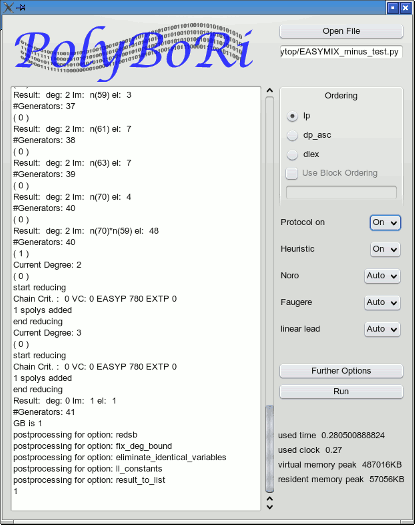
\includegraphics[width=.4\textwidth]{PolyGui}~%
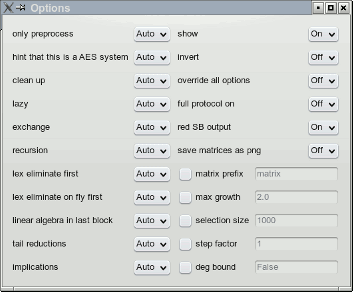
\includegraphics[width=.4\textwidth]{PolyGui-Options}
\caption{PolyGUI:  A graphical user interface for \PolyBoRi's
  \texttt{groebner_basis} command}
\end{figure}


The user make a \Groebner analysis of custom polynomial systems by selecting various options
of \PolyBoRi's \texttt{groebner_basis} command. The ``Open File'' dialog can be
used to load \PolyBoRi-compatible data files. They have to be written in
Python syntax and must contain a ring declaration and the definition of an
\texttt{ideal} (given as a lit of Boolean polynomials).

\paragraph{Example}
\begin{lstlisting}
declare_ring([Block("x", 10), Block("y", 10)])
ideal = [x(1) + x(2), x(2) + y(1)]
\end{lstlisting}

The user interface comes with several switches and buttons which can be used to set
the monomial ordering and the available options of the  \texttt{groebner_basis};
including the protocol  output.
The ``Run'' button is then to be used to execute the \Groebner basis computation.



\subsection{\textsc{Singular}'s pyobject extension}

This approach uses \textsc{Singular}'s upcoming built-in \texttt{pyobject}
extension. For using \PolyBoRi from \textsc{Singular} you must ensure, 
that \PolyBoRi is installed either in the python 
search path, or in \textsc{Singular}'s binary path. PolyBoRi's default installation
target (in the system resources) will work. In case you do not have root access,
you can customize the installation:

\begin{lstlisting}
  scons install PREFIX=/path/to/my/bin PYINSTALLPREFIX=/path/to/python/modules
\end{lstlisting}

where \texttt{/path/to/my/bin} is the users path, and \texttt{/path/to/python/modules}
could be for instance \textsc{Singular}'s binary directory. If you also do not have write
permission to the latter, please add a custom directory to environment
variable \texttt{PYTHONPATH} and use that directory for \texttt{PYINSTALLPREFIX}.

The following session illustrates how \PolyBoRi's functionality can be accessed
from \textsc{Singular}:

\paragraph{Example}
\begin{lstlisting}[language=C]
                     SINGULAR                                 /  Development
 A Computer Algebra System for Polynomial Computations       /   version 3-1-2
                                                           0<
 by: W. Decker, G.-M. Greuel, G. Pfister, H. Schoenemann     \   Oct 2010
FB Mathematik der Universitaet, D-67653 Kaiserslautern        \
// ** executing LIB/.singularrc
> python_import("polybori");
> declare_ring(list(Block("x", 10), Block("y", 10)));
<polybori.dynamic.PyPolyBoRi.Ring object at 0xddf050>
> list polybori_ideal = (x(1)+x(2),x(2)+y(1));
> def result = groebner_basis(polybori_ideal);
> result;
[x(1) + y(1), x(2) + y(1)]
> typeof(result);
pyobject
> result[1];
x(2) + y(1)
> Auf Wiedersehen.
\end{lstlisting}


\begin{thebibliography}{31}

\bibitem{ref1}
Brickenstein, M., 2011. Boolean {Gr{\"{o}}}bner bases -- theory, algorithms and
  applications. Ph.D. thesis, University of Kaiserslautern, Logos Verlag, Berlin,
  Germany, 2011.

\bibitem{ref2}
Brickenstein, M., Dreyer, A., 2010. Network-driven Boolean Normal Forms,
Preprint. 
\newline\url{http://polybori.sourceforge.net/documents/NetworkDriven.pdf}

\bibitem{ref3}
Bulygin, S., Brickenstein, M., 2010. Obtaining and solving systems of equations
  in key variables only for the small variants of {AES}. In: Mathematics in
  Computer Science 3~(2), 185--200.
\newline\url{http://dx.doi.org/10.1007/s11786-009-0020-y}

\bibitem{ref4}
Brickenstein, M., Dreyer, A., 2009. {PolyBoRi}: A framework for
  {Gröbner}-basis computations with {Boolean} polynomials. Journal of Symbolic
  Computation 44~(9), 1326--1345, {Effective Methods in Algebraic Geometry}.
\newline\url{http:/dx.doi.org/10.1016/j.jsc.2008.02.017}

\bibitem{ref5}
Brickenstein, M., Dreyer, A., Greuel, G.-M., Wedler, M., Wienand, O.,
  2009. New developments in the theory of {Gröbner} bases and applications to
  formal verification. Journal of Pure and Applied Algebra 213~(8), 1612--1635,
  {Theoretical Effectivity and Practical Effectivity of Gröbner Bases}.
\newline\url{http://dx.doi.org/10.1016/j.jpaa.2008.11.043}

\bibitem{ref6}
Brickenstein, M., Dreyer, A., 2008.
  Gr\"{o}bner-free normal forms for boolean polynomials.
 In: Proceedings of the twenty-first international symposium on Symbolic and algebraic computation,
 ISSAC '08, Linz/Hagenberg, Austria, 55--62. ACM, New York, NY, USA.
\newline\url{http://doi.acm.org/10.1145/1390768.1390779}

\end{thebibliography}
